\section{Bonus study of parameter estimation with a PINN}
\label{sec:bonus}

\subsection{Inverse problem and synthetic data}

The core simulations use known parameters to predict voltage. Here we reverse the problem and estimate \(a\) from voltage readings alone. We fix \(b=0.80\) and \(\varepsilon=0.08\), supply the current and initial state, and treat recovery \(w\) as unobserved during fitting. The data come from the FHN equations with \(a_{\mathrm{true}}=0.70\), so the parameter error can be measured directly.

We generated clean reference trajectories on \([0,40]\) at intervals of \(0.10\), using DOP853 with relative and absolute tolerances of \(10^{-11}\) and \(10^{-13}\). For the clean training set, we kept every fourth voltage sample, giving 101 observations. For the sparse, noisy set, we chose one positive-time sample per block of ten and added Gaussian noise with standard deviation \(0.03\), giving 40 observations. The two sets sample the same training trajectory.

Training used \(I=0.50\) and \((v_0,w_0)=(-1.15,-0.62)\). Validation used \(I=0.65\) and \((-1.00,-0.55)\). The final test used \(I=0.90\) and \((-1.20,-0.70)\). Only training observations entered either fit.

\begin{figure}[H]
  \centering
  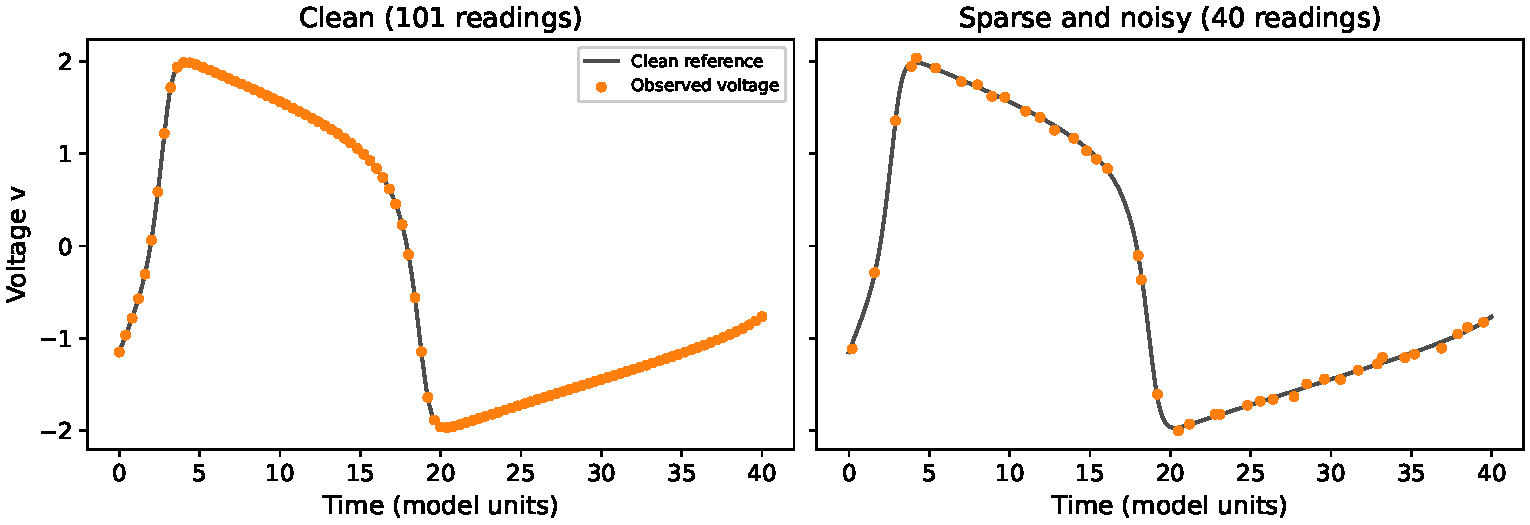
\includegraphics[width=0.83\linewidth]{figures/pinn_training_observations.pdf}
  \caption{The two training datasets. Dots are the supplied observations and the gray curve is the clean numerical reference.}
  \label{fig:pinn-data}
\end{figure}

\clearpage

\subsection{PINN and least-squares fitting}

A physics-informed neural network (PINN) fits observed data while penalizing disagreement with the governing equations \cite{raissi2019}. Our network takes time as input and predicts voltage \(\hat v\) and recovery \(\hat w\). It uses normalized time, three pairs of sine and cosine features, and three hidden layers of 32 units with \(\tanh\) activations. The output takes the form \((\hat v,\hat w)=(v_0,w_0)+(1-e^{-t})N_\theta(t)\), which gives the known initial state exactly at \(t=0\).

At 241 fixed physics times, automatic differentiation supplies the predicted slopes. The residuals are the predicted slopes minus the rates from \eqref{eq:voltage} and \eqref{eq:recovery}, evaluated at the predicted state and fitted \(\hat a\). The objective is
\begin{equation}
  \mathcal{L}
  =\operatorname{mean}_{\rm obs}\!\bigl[(\hat v-v_{\rm obs})^2\bigr]
    +\operatorname{mean}_{\rm grid}\!\bigl[r_v^2+4r_w^2\bigr].
  \label{eq:pinn-loss}
\end{equation}
On a Colab CPU in double precision, we used 400 voltage-only steps, 1800 joint Adam steps, and up to 300 L-BFGS iterations. The data seed was 2026 and the network seed was 7.

The least-squares baseline integrates the FHN model for each trial \(a\) and minimizes squared voltage errors at the same observation times. Both fits start at \(a=0.50\) with the same allowed interval \([0.20,1.20]\).

\subsection{Held-out results}

For validation and testing, we used each fitted \(a\) in the same numerical ODE solver at the new current and initial state. This checks parameter transfer to another trajectory. The voltage error is the root mean square error (RMSE) against the corresponding clean reference. Relative parameter error is \(100|\hat a-a_{\mathrm{true}}|/|a_{\mathrm{true}}|\).

\begin{table}[H]
  \centering
  \caption{Parameter recovery and final-test errors at \(I=0.90\). Entries shown as zero are rounded to the displayed precision.}
  \label{tab:pinn-test}
  \small
  \setlength{\tabcolsep}{5pt}
  \begin{tabular}{llrrrr}
    \toprule
    Training data & Method & \(\hat a\) & Rel.\ error & Voltage RMSE & Recovery RMSE\\
    \midrule
    Clean & PINN          & 0.699975 & \(0.0036\%\) & 0.000096 & 0.000022\\
    Clean & Least squares & 0.700000 & \(0.00\%\)   & 0.000000 & 0.000000\\
    Sparse, noisy & PINN          & 0.704093 & \(0.58\%\) & 0.015570 & 0.003554\\
    Sparse, noisy & Least squares & 0.701926 & \(0.28\%\) & 0.007343 & 0.001677\\
    \bottomrule
  \end{tabular}
\end{table}

\begin{figure}[H]
  \centering
  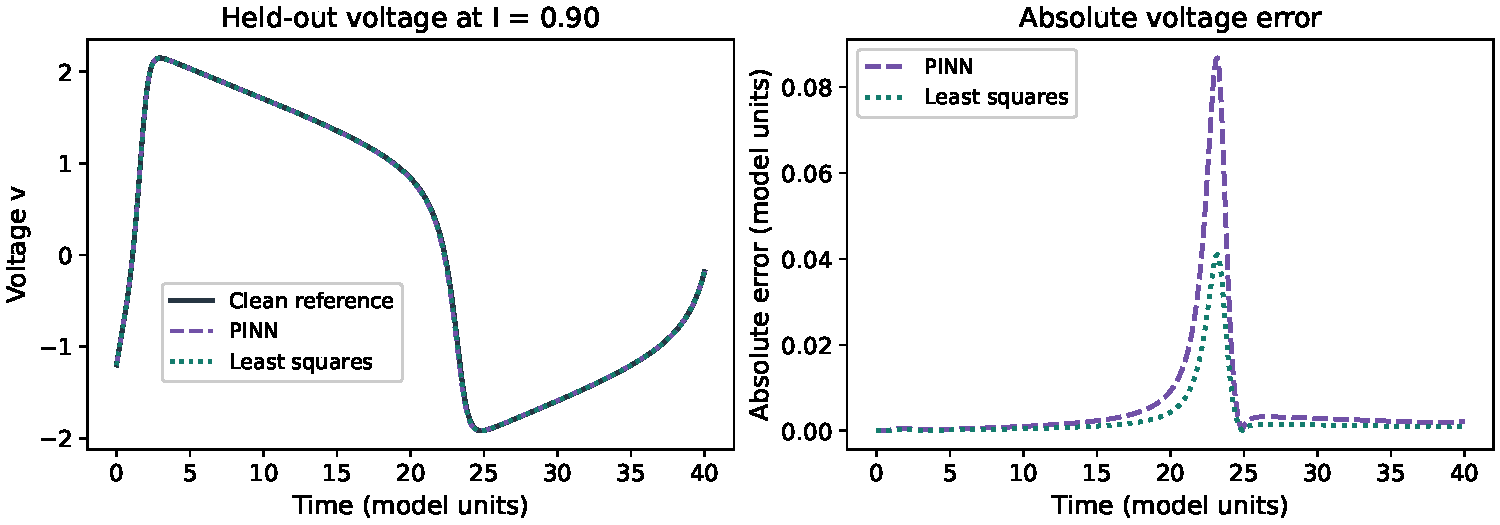
\includegraphics[width=0.91\linewidth]{figures/pinn_heldout_comparison.pdf}
  \caption{Final-test voltages and absolute errors for the sparse, noisy fits. The curves are regenerated from the fitted parameters rounded to six decimal places.}
  \label{fig:pinn-test}
\end{figure}

Both methods matched the single reference spike in the final test. On noisy validation data, voltage RMSE was \(0.011649\) for the PINN and \(0.005491\) for least squares.
